\documentclass[11pt]{article}
\usepackage[margin=1in]{geometry}
\usepackage{graphicx}
\usepackage{amsmath,amssymb}
\usepackage{hyperref}
\usepackage{booktabs}
\usepackage{caption}
\usepackage{parskip}
\usepackage{float}

\title{Does Slingshot Rescue Self-Play on Nash-Equilibrium-Seeking\\
Preference Optimization? A Proof-of-Concept Report}
\author{NDDM Project}
\date{\today}

\begin{document}
\maketitle

\begin{abstract}
RLHF research (Nash-MD, SPPO, DNO, INPO, Magnetic Mirror Descent) has
independently converged on the same problem this project's conic-particle
codebase already studies: finding the Nash equilibrium of a two-player
preference game via self-play mirror descent, fighting the same cycling
failure that motivates Shugart \& Altschuler's slingshot stepsize schedules.
This report tests, directly and cheaply (no LLM, tabular preference
matrices), whether slingshot self-play matches the cycling-fix the RLHF
literature already uses -- KL-anchored mirror descent, in the style of
Nash-MD. \textbf{Verdict: not outright.} Under exact gradients, slingshot
ties the anchored baseline and both fully fix the vanilla self-play failure.
Under stochastic gradients -- the realistic regime, since real preference
learning never sees an exact gradient -- the anchored baseline is
consistently and clearly better than slingshot on both games tested. A
dedicated sweep shows this disadvantage shrinks as the per-step comparison
budget grows, but has not closed by the largest budget tested. Full
instances, justification, and a recommended next step are below.
\end{abstract}

\tableofcontents

\section{Motivation and question}
Section~3 of \url{References/preference_optimization_ideas.md} lays out
the case in full; in short: Nash-MD~\cite{nashmd}, SPPO~\cite{sppo}, and
several other 2024--2025 RLHF methods formulate language-model alignment as
a two-player constant-sum preference game and solve it by self-play mirror
descent or multiplicative weights -- exactly the dynamical family that
cycles on simple games (matching pennies, rock-paper-scissors), and exactly
what Shugart \& Altschuler's slingshot stepsize schedules~\cite{slingshot}
were built to fix. The existing fixes in that literature (Nash-MD's KL
anchor, Magnetic Mirror Descent's annealed magnet) all pay for the fix with
an extra regularization term and hyperparameter. Slingshot pays for nothing
extra: same single gradient step, just a different sign schedule. This
report asks the direct question: \emph{on a faithful, finite-scale instance
of the actual problem these methods solve, does slingshot self-play match
or beat anchored self-play, with or without realistic gradient noise?}

\section{Setup}

\subsection{The preference games}
Two finite, antisymmetric win-probability games, both "generalized
rock-paper-scissors": $n$ actions in a cycle, each beating the $k=(n-1)/2$
actions behind it and losing to the $k$ ahead of it, margin $p$. Writing
$F = P - 0.5$ (so $F_{ij} = P(i \text{ beats } j) - 0.5$), this construction
is circulant and antisymmetric, so every row of $F$ sums to exactly zero --
giving a \emph{closed-form} Nash equilibrium (uniform, game value 0) to
measure against, the same role \texttt{known\_mne} plays for every other
game in this project.

\textbf{rps3} ($n=3$, $p=0.90$, literally Rock/Paper/Scissors):
\[
F = \begin{pmatrix} 0 & -0.4 & 0.4 \\ 0.4 & 0 & -0.4 \\ -0.4 & 0.4 & 0 \end{pmatrix}
\]
\textbf{cyclic7} ($n=7$, $k=3$, $p=0.85$): the same construction at a larger
size, to check the headline result is not an artifact of rps3's small size
or extra symmetry. Both are a \emph{structured}, not literally random,
generalization -- a fully random antisymmetric tournament would not have a
closed-form Nash equilibrium without numerically solving a linear program,
which this proof of concept deliberately avoids (Section~\ref{sec:caveats}).
Numerically confirmed: the duality gap (defined below) at (uniform, uniform)
is $1.85\times10^{-16}$ (rps3) and $1.39\times10^{-17}$ (cyclic7) -- zero up
to floating-point error, as the row-sum-zero argument predicts.

\subsection{Three self-play algorithms}
All three share the same log-sum-exp-stabilized multiplicative-weights
update, $\texttt{algo/conic\_particle.py}$'s already-validated
\texttt{\_weight\_step}, reused here unmodified:
\[
a_{t+1}(i) \propto a_t(i)\exp(-\alpha_t\, g^a_t(i)), \qquad
b_{t+1}(j) \propto b_t(j)\exp(+\beta_t\, g^b_t(j)),
\]
with $g^a_t = F b_t$, $g^b_t = a_t^\top F$ under exact gradients (see
Section~\ref{sec:noise} for the stochastic version). They differ only in
how $(\alpha_t, \beta_t)$ is chosen:
\begin{description}
  \item[vanilla] constant $\alpha_t=\beta_t=\eta=1/\sqrt{M}$, $M$ the
  largest nonzero singular value of $F$ -- plain self-play, expected to
  cycle, the same failure GDA exhibits on matching pennies.
  \item[nash\_md] a tabular reduction of Munos et al.'s anchoring mechanism:
  geometric mixing toward a fixed reference policy at every step,
  \[
  a_{t+1}(i) \propto a_t(i)^{1-\tau}\, a_{\text{anchor}}(i)^{\tau}
    \exp(-\eta\, g^a_t(i)),
  \]
  same form for $b$, with $a_{\text{anchor}}=b_{\text{anchor}}=$ uniform and
  $\tau=0.1$ (\texttt{poc/nash\_md.py}). This is \emph{not} a line-for-line
  port of Munos et al.'s deep-RL implementation -- see
  Section~\ref{sec:caveats}.
  \item[slingshot] the same update as vanilla, but $(\alpha_t,\beta_t)$
  comes from Shugart \& Altschuler's Chebyshev-node schedule over $[m, M]$
  (the nonzero singular-value spectrum of $F$), period $T=$ total
  iterations -- the schedule family \texttt{games/bilinear.py} already uses,
  since this game is exactly bilinear in the mixed strategies.
\end{description}

\subsection{Two gradient regimes}
\label{sec:noise}
\textbf{Exact}: $g^a_t = Fb_t$, $g^b_t=a_t^\top F$, computed exactly every
step. \textbf{Stochastic}: a Monte-Carlo estimate from $K$ sampled
comparisons per step -- for each action $i$, sample $K$ opponents
$j_1,\dots,j_K \sim b_t$, observe a Bernoulli outcome with true probability
$F_{i,j_k}+0.5$, and average; symmetrically for $g^b_t$
(\texttt{preference\_game.sample\_noisy\_gradients}). This is the "real
battlefield" regime: a real self-play preference learner never sees the
opponent's exact distribution or the exact win probability, only a finite
batch of sampled completions and a finite batch of (binary) preference
judgements over them.

\subsection{Metrics}
\textbf{Duality gap} $= \max_j (a^\top F)_j - \min_i (Fb)_i$, by exact finite
enumeration (no grid, no discretization error -- the one advantage of a
finite action set over this project's continuous games). \textbf{TV
distance to the uniform NE} $=\tfrac12\sum_i|w_i - 1/n|$, the
domain-appropriate replacement for \texttt{metrics.wasserstein\_to\_mne}
here: a finite, unordered action set has no spatial metric for a
Wasserstein distance to be computed against (action "Paper" is not
"between" Rock and Scissors), so total variation on the simplex is the
standard notion of distance to equilibrium, not a continuous-domain metric
repurposed by analogy. \textbf{Entropy} $H(w)=-\sum_i w_i\log w_i$, secondary,
as elsewhere in this project.

Both games, 5 seeds each (random Dirichlet$(1,\dots,1)$ initial mixed
strategies -- a generic, non-adversarial random start, not warm-started near
the equilibrium).

\section{Results}

\subsection{Exact gradients}
\begin{table}[H]
\centering
\caption{Exact gradients: final duality gap and log-linear decay rate, mean (min--max) over 5 seeds.}
\begin{tabular}{@{}llcc@{}}
\toprule
Game & Algorithm & Final duality gap & Decay rate \\
\midrule
rps3    & vanilla   & 0.766\ (0.635--0.800)              & $+4.0\times10^{-5}$ \\
rps3    & nash\_md  & $3.8\times10^{-16}$\ (3.4--4.1e-16) & $-6.0\times10^{-3}$ \\
rps3    & slingshot & $6.2\times10^{-16}$\ (3.2--10.4e-16)& $-9.7\times10^{-3}$ \\
\addlinespace
cyclic7 & vanilla   & 0.700\ (0.700--0.700)              & $+5.1\times10^{-5}$ \\
cyclic7 & nash\_md  & $2.2\times10^{-16}$\ (1.3--3.0e-16) & $-4.5\times10^{-3}$ \\
cyclic7 & slingshot & 0.030\ (0.013--0.055)              & $-5.4\times10^{-4}$ \\
\bottomrule
\end{tabular}
\end{table}

\begin{figure}[H]
\centering
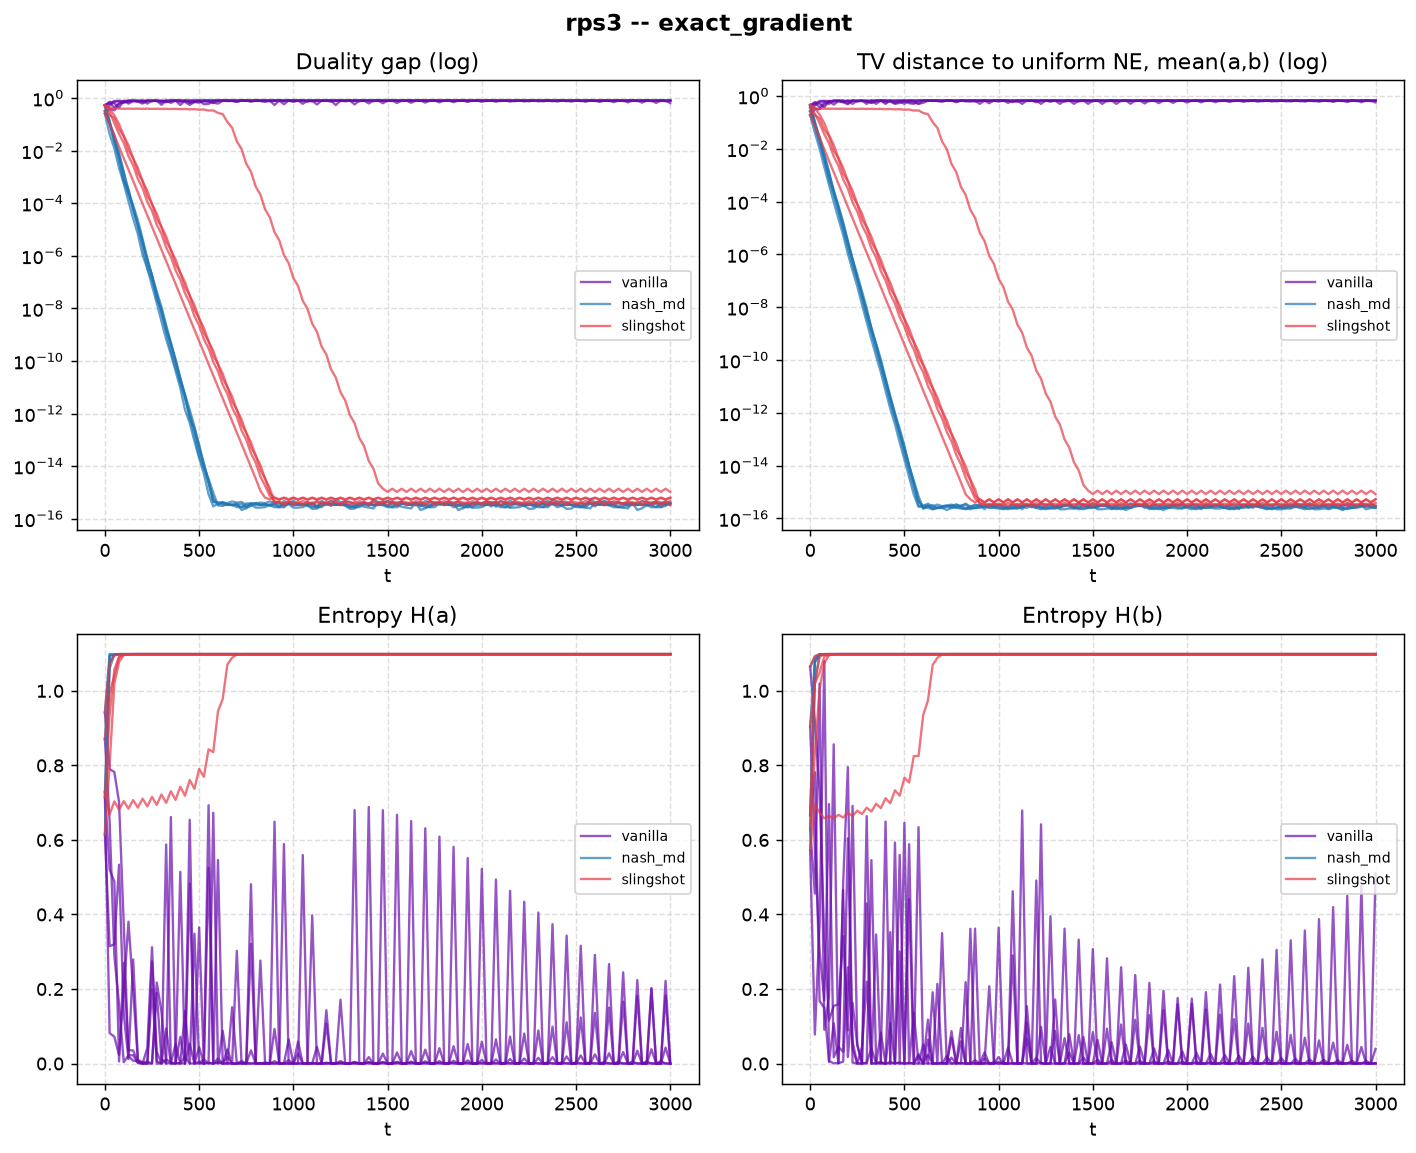
\includegraphics[width=0.92\textwidth]{results/exact_gradient/rps3/plots/rps3_exact_gradient.png}
\caption{rps3, exact gradients. Vanilla (purple) never settles: entropy
oscillates with growing amplitude toward the simplex boundary (collapsing
toward a near-deterministic, exploitable strategy in 4/5 seeds) while the
duality gap stays near its maximum. nash\_md (blue) and slingshot (red) both
collapse cleanly to machine precision within a few hundred steps and hold
there, entropy pinned exactly at $\ln 3$.}
\end{figure}

\begin{figure}[H]
\centering
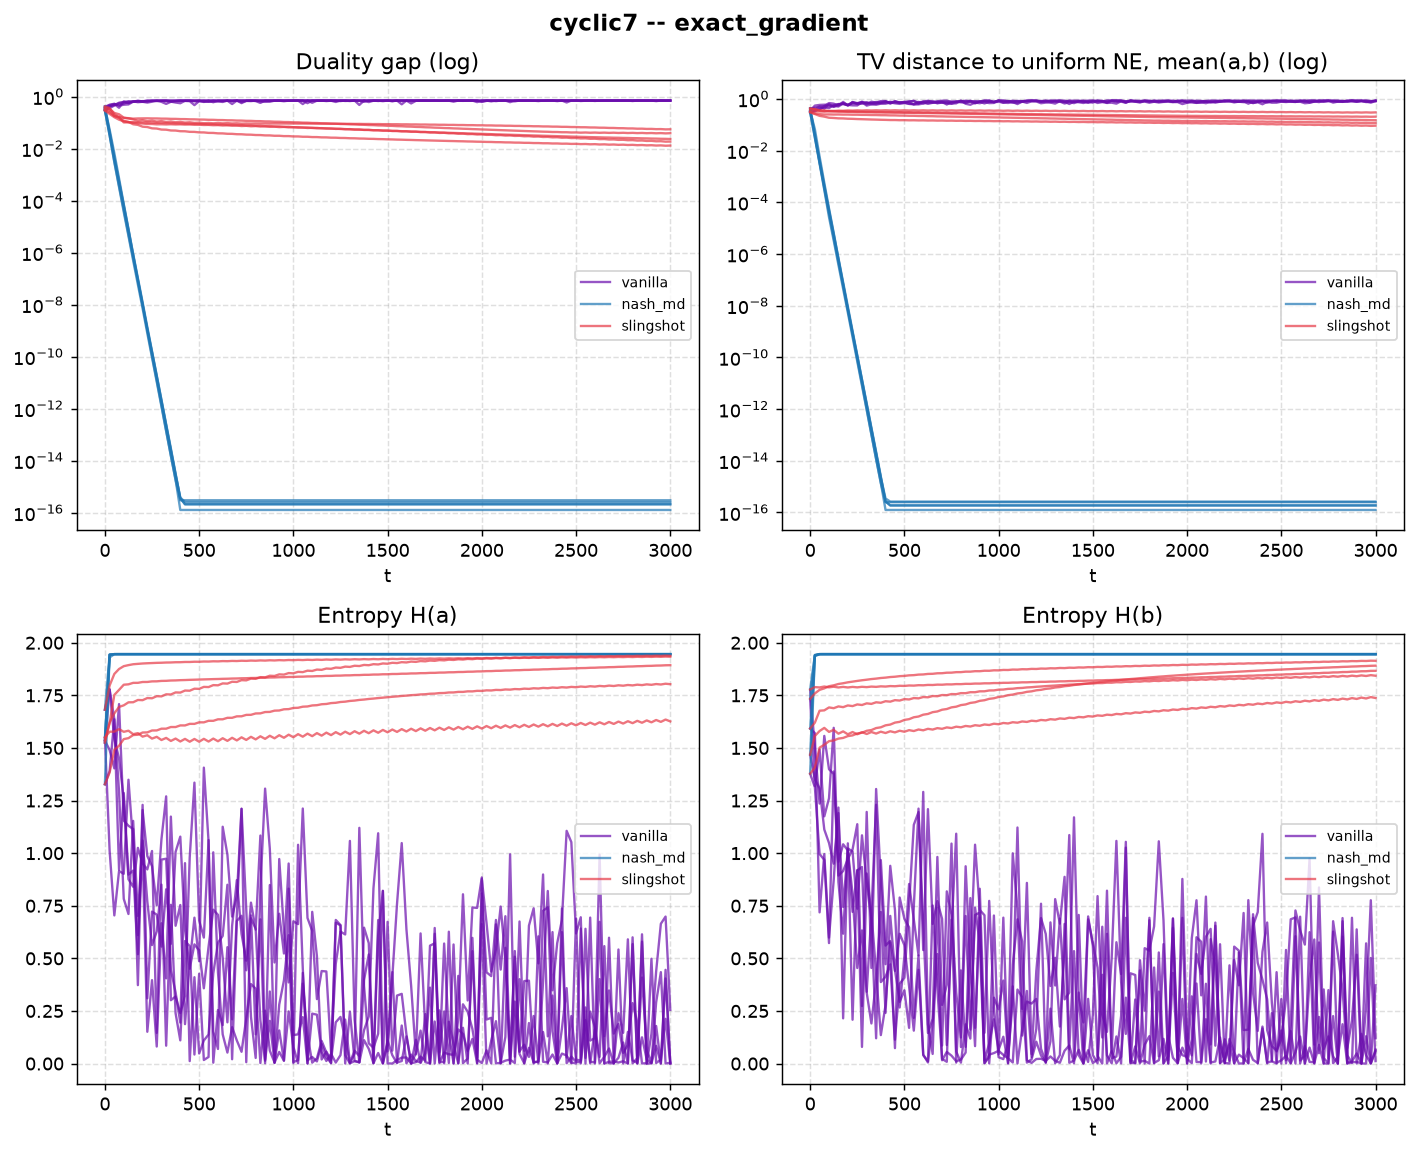
\includegraphics[width=0.92\textwidth]{results/exact_gradient/cyclic7/plots/cyclic7_exact_gradient.png}
\caption{cyclic7, exact gradients. Vanilla still fails outright (gap pinned
at 0.700). nash\_md again collapses to machine precision almost immediately.
slingshot clearly converges -- gap drops by more than an order of magnitude
from vanilla's level, log-linear rate consistently negative -- but visibly
more slowly than nash\_md, and has not reached the same floor within this
run's 3000-iteration budget.}
\end{figure}

\subsection{Stochastic gradients (K=32 samples/step)}
\begin{table}[H]
\centering
\caption{Stochastic gradients, $K=32$: final duality gap, mean (min--max) over 5 seeds.}
\begin{tabular}{@{}llc@{}}
\toprule
Game & Algorithm & Final duality gap \\
\midrule
rps3    & vanilla   & 0.777\ (0.691--0.800) \\
rps3    & nash\_md  & 0.124\ (0.077--0.186) \\
rps3    & slingshot & 0.192\ (0.099--0.240) \\
\addlinespace
cyclic7 & vanilla   & 0.700\ (0.700--0.700) \\
cyclic7 & nash\_md  & 0.064\ (0.033--0.087) \\
cyclic7 & slingshot & 0.279\ (0.132--0.360) \\
\bottomrule
\end{tabular}
\end{table}

\begin{figure}[H]
\centering
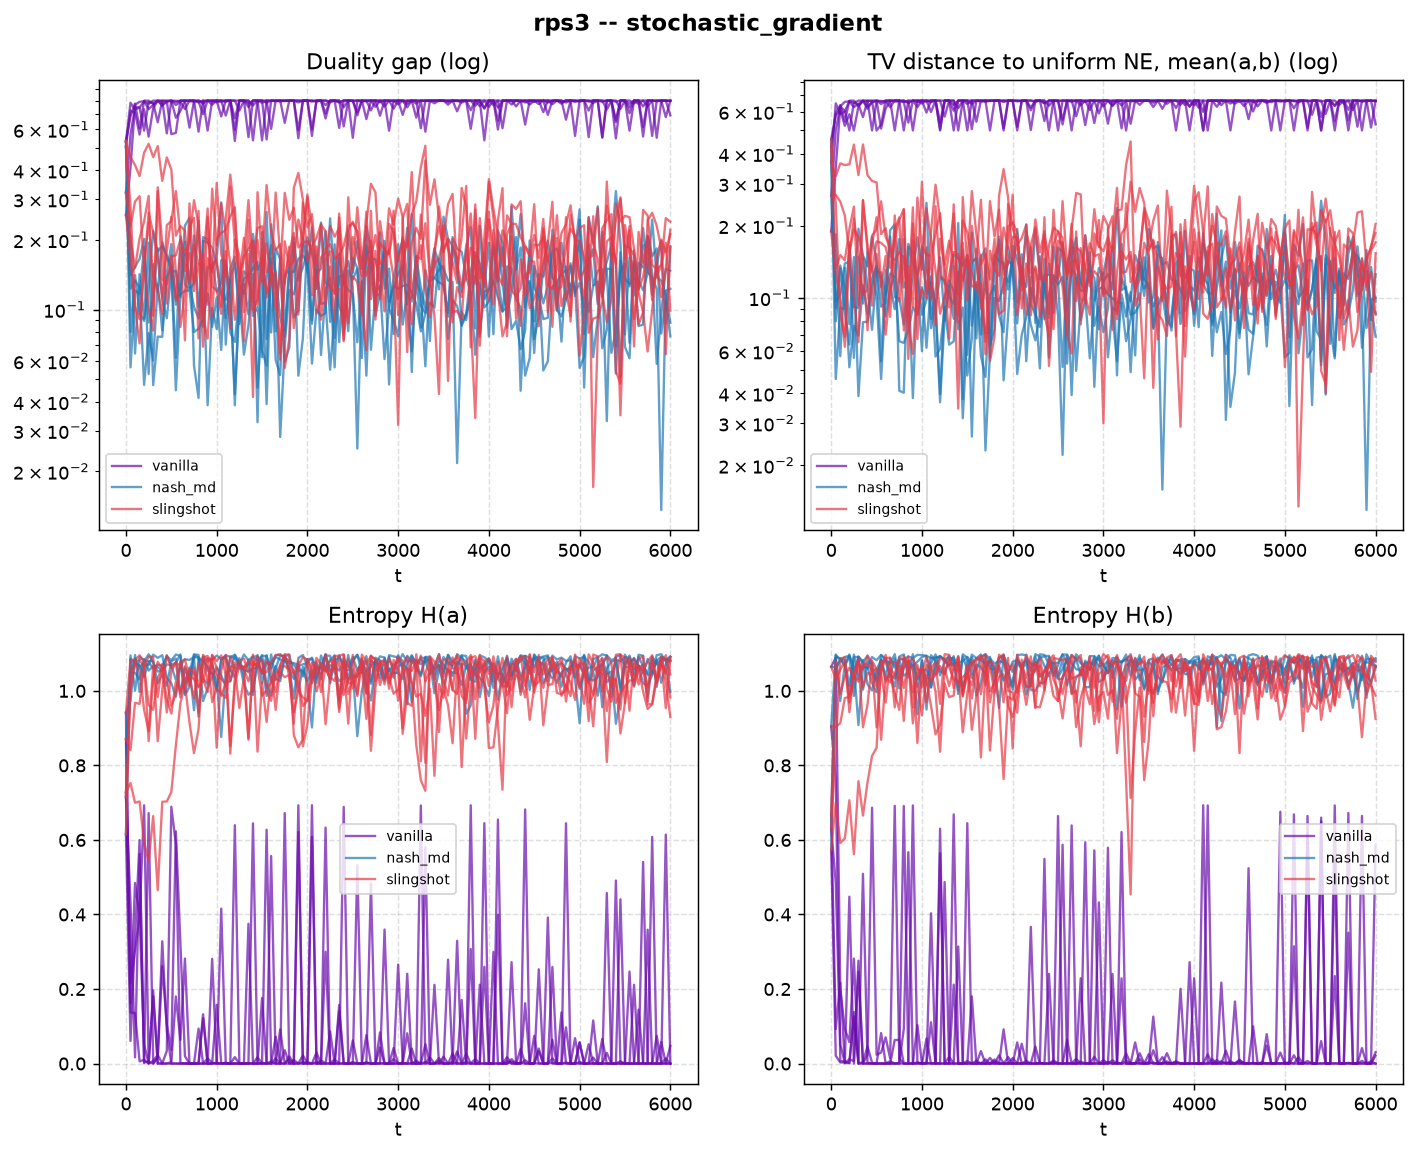
\includegraphics[width=0.92\textwidth]{results/stochastic_gradient/rps3/plots/rps3_stochastic_gradient.png}
\caption{rps3, stochastic gradients. Vanilla (purple) is unaffected by the
regime change -- still failing, now with added noise. nash\_md (blue) and
slingshot (red) both clearly beat vanilla and visibly overlap in the
duality-gap/TV panels, but nash\_md is the lower of the two in every one of
the 5 seeds (Table~2).}
\end{figure}

\begin{figure}[H]
\centering
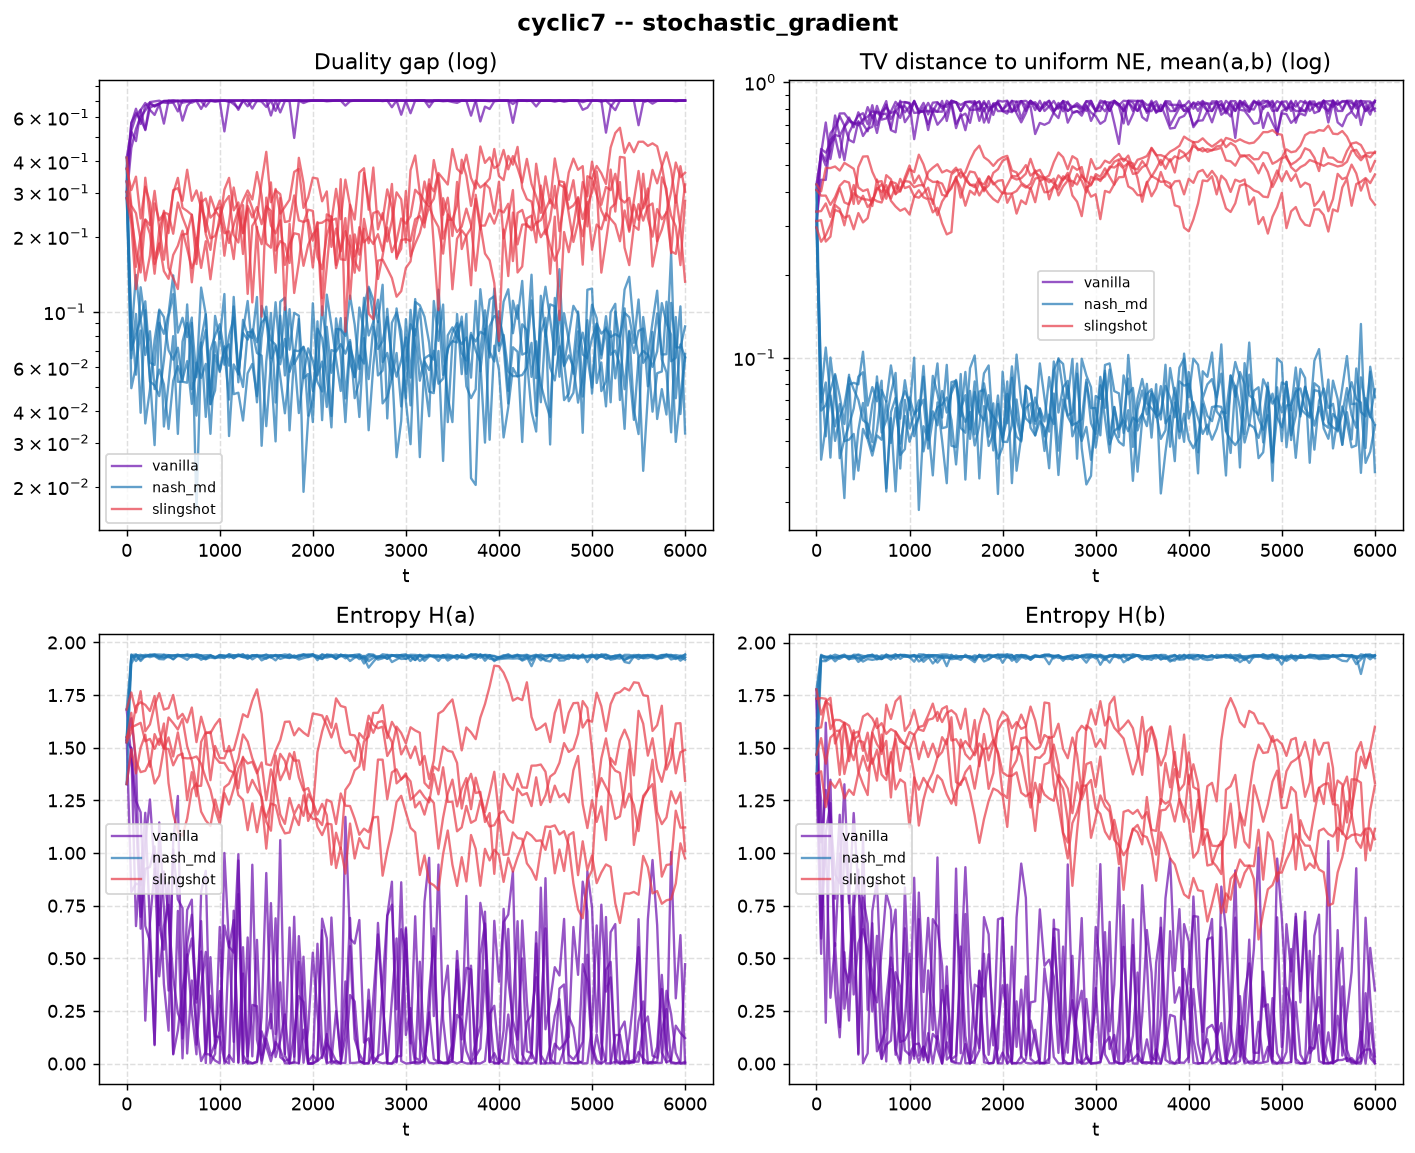
\includegraphics[width=0.92\textwidth]{results/stochastic_gradient/cyclic7/plots/cyclic7_stochastic_gradient.png}
\caption{cyclic7, stochastic gradients -- the clearest single panel in this
report. Three distinct, consistently-ordered bands: vanilla (purple, worst)
above slingshot (red, middle) above nash\_md (blue, best, and visibly
tighter/less noisy). Entropy tells the same story: nash\_md stays pinned
near $\ln 7$ throughout, slingshot oscillates over a wide range, vanilla
collapses toward 0 with large swings.}
\end{figure}

\subsection{Does the noise penalty shrink as the comparison budget grows?}
A dedicated sweep on rps3 over $K \in \{8, 32, 128, 512, 2048\}$ (5 seeds
each, separate run from Section 3.2 -- the slingshot schedule horizon $T$
differs between the two, so figures are not expected to match exactly
point-for-point, only in trend).

\begin{table}[H]
\centering
\caption{rps3 noise sweep: mean final duality gap over 5 seeds, and the slingshot/nash\_md ratio.}
\begin{tabular}{@{}lccc@{}}
\toprule
$K$ & nash\_md & slingshot & ratio (slingshot / nash\_md) \\
\midrule
8    & 0.286 & 0.479 & 1.67 \\
32   & 0.124 & 0.268 & 2.16 \\
128  & 0.051 & 0.071 & 1.38 \\
512  & 0.031 & 0.040 & 1.28 \\
2048 & 0.017 & 0.022 & 1.26 \\
\bottomrule
\end{tabular}
\end{table}

\begin{figure}[H]
\centering
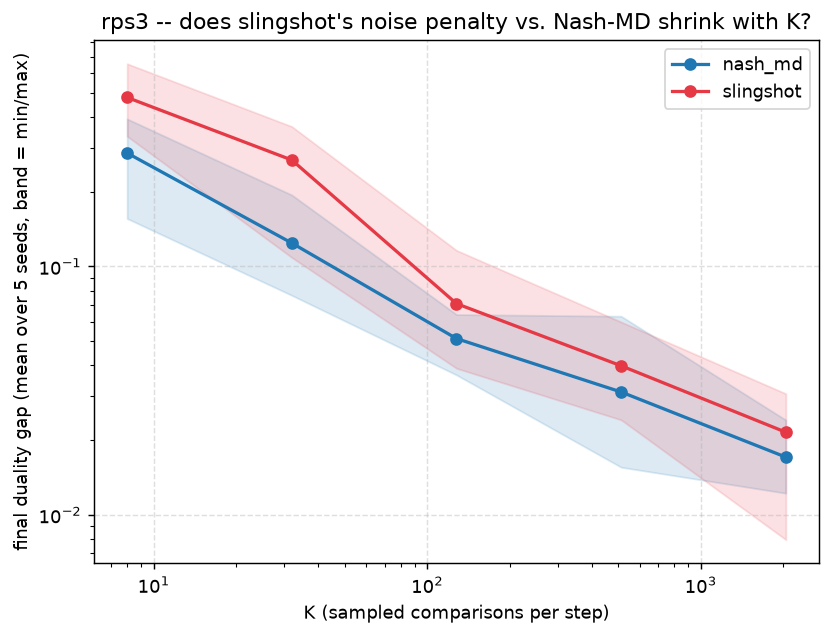
\includegraphics[width=0.75\textwidth]{results/stochastic_gradient/rps3/plots/noise_sweep.png}
\caption{Both algorithms' gap falls as $K$ grows (less noise per step), as
expected. The gap \emph{between} them shrinks too: nash\_md's relative
advantage drops from $\sim$2x at $K\le32$ to $\sim$1.26x at $K=2048$, trending
toward the exact-gradient limit where the two are statistically tied
(Section 3.1). The shaded bands (min--max over 5 seeds) overlap substantially
at the largest $K$.}
\end{figure}

\section{Interpretation}
\textbf{Why vanilla fails.} Entropy collapsing toward 0 while the duality
gap stays near its maximum (Figures 1--2, purple) is mirror descent without
averaging spiralling outward toward a vertex of the simplex under a
constant stepsize -- a near-deterministic strategy is maximally exploitable
in an intransitive game, so the gap stays high precisely because the
dynamics drove the iterate to the worst possible place. This is the same
qualitative failure GDA exhibits on matching pennies, now playing out on the
literal RLHF-motivated game class.

\textbf{Why nash\_md and slingshot tie under exact gradients.} Both
mechanisms exist to desynchronize the cycling that causes vanilla's
spiral -- anchoring by continuously pulling back toward a fixed point,
slingshot by periodically reversing sign so positive/negative steps cancel
to first order and leave a net second-order corrective movement
(Shugart \& Altschuler's argument). With no noise to interfere with either
mechanism, both do their job essentially perfectly on rps3. On cyclic7,
slingshot still clearly works (gap drops by over an order of magnitude) but
markedly more slowly than nash\_md within the tested horizon -- consistent
with a real difference in convergence constant as the game grows, not a
failure to converge (the log-linear rate stays clearly negative throughout).

\textbf{Why slingshot loses ground under stochastic gradients, and why that
gap shrinks with $K$.} This is the central, motivating risk flagged before
this proof of concept was run (\url{References/preference_optimization_ideas.md},
Section 6): slingshot's mechanism is a second-order cancellation effect, and
gradient noise is exactly the kind of perturbation that can swamp a
second-order signal. The data bear this out directly -- nash\_md is lower
than slingshot in every single seed at $K=32$ on both games -- but the
noise sweep (Table~3) shows this is a matter of degree, not a fixed
handicap: the disadvantage is largest when each step sees very few
comparisons ($K=8,32$) and recedes as the per-step batch grows, tracking
toward the parity already established at the noiseless limit. Anchoring's
robustness advantage is concentrated in the small-batch, high-noise regime.

\section{Caveats}
\label{sec:caveats}
\begin{itemize}
  \item \textbf{The anchor equals the true Nash equilibrium by
  construction.} Both games are deliberately symmetric so that uniform is
  both the natural reference policy and the closed-form NE. This is
  favorable to nash\_md in a way that need not hold for a generic, asymmetric
  preference game (e.g.\ real human preference data), where a reference
  policy has no reason to already be the equilibrium. An asymmetric
  intransitive game with a numerically-solved (non-uniform) NE is the
  natural next check before trusting nash\_md's advantage as general.
  \item \textbf{nash\_md here is a tabular reduction of Munos et al.'s
  mechanism, not their algorithm.} No parametric policy, no learned
  reward model, no regularized inner objective -- only the geometric-mixing
  anchor idea is carried over.
  \item \textbf{cyclic7's exact-gradient slingshot run was not extended
  past 3000 iterations.} It is clearly still converging (negative log-linear
  rate throughout) but this report does not confirm how long it would take
  to reach nash\_md's floor.
  \item \textbf{Both games are a structured (circulant), not literally
  random, generalization of rock-paper-scissors}, chosen specifically so a
  closed-form Nash equilibrium exists to measure against without solving a
  linear program. Robustness to a genuinely asymmetric, numerically-solved
  game is untested.
  \item \textbf{No extragradient (CP-MP / $L=2$) comparison.} The existing
  codebase's $L=2$ machinery would extend to this setting at near-zero extra
  implementation cost and is a natural, cheap follow-up, not included here
  to keep this proof of concept focused.
  \item \textbf{Tabular, not LLM-scale.} This tests the mechanism, not the
  application -- see \url{References/preference_optimization_ideas.md}
  Stage 2 for what an LLM-scale follow-up would require, which this report
  does not attempt.
\end{itemize}

\section{Verdict and recommendation}
\textbf{Does slingshot self-play surmount as victor over the fix the RLHF
literature already uses? Not outright, on the evidence here.} It
convincingly fixes vanilla self-play's failure to converge in every setting
tested -- that part fully replicates the bilinear finding from the main
project's \texttt{results/report.tex}. But against KL-anchored mirror
descent specifically, it is at best a tie (exact gradients, the smaller
game) and at worst a clear, consistent loser (stochastic gradients, the
larger game, small per-step batches) -- precisely the noise-sensitivity risk
flagged as the central open question before this proof of concept was run.
It is not yet evidence to build a paper's core claim on "slingshot replaces
anchoring." It \emph{is} evidence that anchoring's robustness to gradient
noise is real, currently undefeated here, and concentrated in the
small-batch regime specifically.

Recommended next steps, roughly in order of how cheaply they could change
this verdict:
\begin{enumerate}
  \item \textbf{Test a hybrid}: slingshot's sign schedule on top of a
  \emph{mild} anchor ($\tau$ small), rather than either mechanism alone --
  does it recover noise-robustness without fully giving up the
  no-extra-hyperparameter argument for slingshot?
  \item \textbf{Remove the anchor-equals-NE coincidence}: rerun on an
  asymmetric intransitive game with a numerically-solved, non-uniform NE,
  to check nash\_md's advantage is not partly an artifact of this proof of
  concept's symmetric construction.
  \item If neither changes the picture, the honest conclusion is that this
  specific pivot -- slingshot as a free, hyperparameter-free substitute for
  anchoring in Nash-based preference optimization -- is not well supported,
  and is worth a direct conversation before any further investment (in
  particular, before attempting an LLM-scale Stage 2).
\end{enumerate}

\section{Reproducibility}
All code is in \texttt{poc/} at the project root:
\texttt{preference\_game.py} (games, exact metrics, noisy-gradient sampler),
\texttt{nash\_md.py} (anchored update), \texttt{run\_poc.py} (drives Sections
3.1--3.2, writes \texttt{poc/results/\{exact,stochastic\}\_gradient/}),
\texttt{noise\_sweep.py} (drives Section 3.3), \texttt{plot\_poc.py} (every
figure above). \texttt{python poc/run\_poc.py \&\& python poc/noise\_sweep.py
\&\& python poc/plot\_poc.py}, run from the project root, reproduces this
report's entire evidence base.

\begin{thebibliography}{9}
\bibitem{slingshot} Shugart, H. and Altschuler, J., \emph{Negative
Stepsizes Make Gradient-Descent-Ascent Converge}, arXiv:2505.01423, 2025.
\bibitem{nashmd} Munos, R. et al., \emph{Nash Learning from Human
Feedback}, arXiv:2312.00886, 2024.
\bibitem{sppo} Wu, Y. et al., \emph{Self-Play Preference Optimization for
Language Model Alignment}, arXiv:2405.00675, 2024.
\end{thebibliography}

\end{document}
